\documentclass{article}
    
    \usepackage{graphicx} % Used to insert images
    \usepackage{adjustbox} % Used to constrain images to a maximum size 
    \usepackage{color} % Allow colors to be defined
    \usepackage{enumerate} % Needed for markdown enumerations to work
    \usepackage{geometry} % Used to adjust the document margins
    \usepackage{amsmath} % Equations
    \usepackage{amssymb} % Equations
    \usepackage{eurosym} % defines \euro
    \usepackage[mathletters]{ucs} % Extended unicode (utf-8) support
    \usepackage[utf8x]{inputenc} % Allow utf-8 characters in the tex document
    \usepackage{fancyvrb} % verbatim replacement that allows latex
    \usepackage{grffile} % extends the file name processing of package graphics 
                         % to support a larger range 
    % The hyperref package gives us a pdf with properly built
    % internal navigation ('pdf bookmarks' for the table of contents,
    % internal cross-reference links, web links for URLs, etc.)
    \usepackage{hyperref}
    \usepackage{longtable} % longtable support required by pandoc >1.10
    \usepackage{booktabs}  % table support for pandoc > 1.12.2
    \usepackage{indentfirst}
    \usepackage{floatrow}
    \usepackage{relsize}
    \usepackage{multirow}
        
    \newcommand\perm[2]{{}_{#1}P_{#2}}%
    \newcommand\todo[1]{\textbf{TODO: #1}}% 
    \newcommand\numberthis{\addtocounter{equation}{1}\tag{\theequation}}
    \newcommand\seteq{\mathrel{\overset{\makebox[0pt]{\mbox{\normalfont\small\sffamily set}}}{=}}}
    \newcommand\mfrac[2]{\left(\dfrac{#1}{#2}\right)}
    \newcommand\lint{\mathlarger{\int}}
    \newcommand\lsum{\mathlarger{\sum}}
    
    \title{Homework 11}
    \author{Roly Vicar\'ia \\ STAT414 Spring 2016}
    
\begin{document}
    
    \maketitle
    
    \textbf{Section 4.3}
    \begin{enumerate}
     %1
     \item 
      \begin{enumerate}
       %a
       \item
	Joint and marginal pmfs:
	\begin{figure}[h!]
	  \centering
	  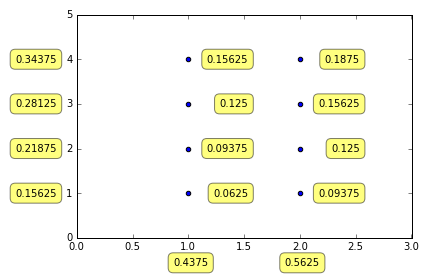
\includegraphics[scale=.6,keepaspectratio=true]{./images/1a_joint_probability_plot.png}
	  % 1a_joint_probability_plot.png: 430x280 pixel, 96dpi, 11.38x7.41 cm, bb=0 0 322 210
	\end{figure}
       
       \newpage
       %b
       \item
	We are given that $f(x,y) = \dfrac{x+y}{32}, x=1,2\ \ y=1,2,3,4$. In order to find $g(x|y)$,
	we start by finding $f_Y(y)$:
	  \begin{align*}
	   f_Y(y) &= \mathlarger{\sum}_{x\in\{1,2\}}{\dfrac{x+y}{32}} \\
	    &= \dfrac{1+y}{32} + \dfrac{2+y}{32} \\
	    &= \dfrac{2y + 3}{32}
	  \end{align*}

	Therefore, the conditional pmf of $X$, given that $Y = y$, is:
	  \begin{align*}
	   g(x|y) = \dfrac{(x+y)/32}{(2y+3)/32} = \dfrac{x+y}{2y+3}, 
		x=1,2,\ \text{when}\ y=1,2,3,\ \text{or}\ 4
	  \end{align*}
	  
	\begin{figure}[h!]
	  \centering
	  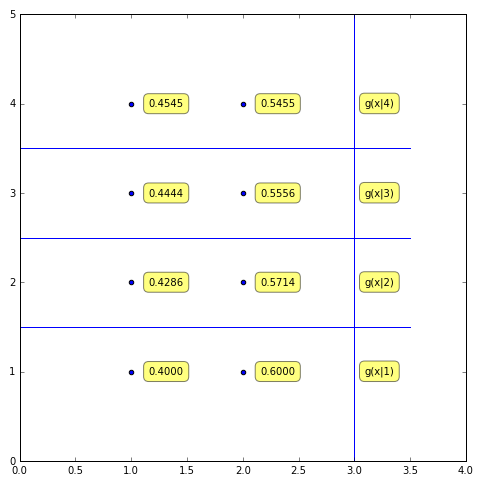
\includegraphics[scale=.6,keepaspectratio=true]{./images/1b_conditional_pmf_plot.png}
	  % 1b_conditional_pmf_plot.png: 486x485 pixel, 96dpi, 12.86x12.83 cm, bb=0 0 364 364
	\end{figure}
       
       %c
       \item
	We start by finding $f_X(x)$:
	  \begin{align*}
	   f_X(x) &= \mathlarger{\sum}_{y\in\{1,2,3,4\}}{\dfrac{x+y}{32}} \\
	    &= \dfrac{x+1}{32} + \dfrac{x+2}{32} + \dfrac{x+3}{32} + \dfrac{x+4}{32} \\
	    &= \dfrac{4x + 10}{32} \\
	    &= \dfrac{2x+5}{16}
	  \end{align*}

	Therefore, the conditional pmf of $Y$, given that $X = x$, is:
	  \begin{align*}
	   h(y|x) &= \dfrac{(x+y)/32}{(2x+5)/16} \\
	    &= \dfrac{x+y}{4x+10}, y=1,2,3,4\ \text{when}\ x=1\ \text{or}\ 2.
	  \end{align*}
	  
	\begin{figure}[h!]
	  \centering
	  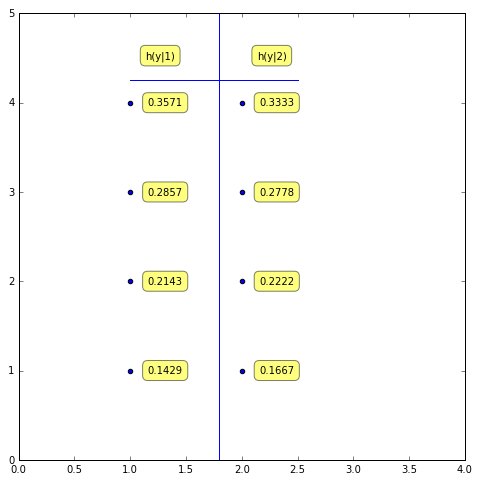
\includegraphics[scale=.6,keepaspectratio=true]{./images/1c_conditional_pmf_plot.png}
	  % 1c_conditional_pmf_plot.png: 484x484 pixel, 96dpi, 12.80x12.80 cm, bb=0 0 363 363
	\end{figure}
       
       %d
       \item
	$P(1 \le Y \le 3 | X = 1) = \dfrac{1+1}{4(1)+10} + \dfrac{1+2}{4(1)+10} + \dfrac{1+3}{4(1)+10}
	  = \dfrac{9}{14}$ \\
	  
	$P(Y \le 2|X=2) = \dfrac{2+1}{4(2)+10} + \dfrac{2+2}{4(2)+10} = \dfrac{7}{18}$ \\
	
	$P(X=2|Y=3) = \dfrac{2+3}{2(3)+3} = \dfrac{5}{9}$
       
       %e
       \item
	$E(Y | X=1) = \mathlarger{\sum}_{y=1}^4{y \dfrac{1+y}{4(1)+10}}
	  = (1)\dfrac{1+1}{14} + (2)\dfrac{1+2}{14} + (3)\dfrac{1+3}{14} + (4)\dfrac{1+4}{14}
	  = \dfrac{40}{14} = \dfrac{20}{7}$ \\
	
	\begin{align*}
	Var(Y|X=1) &= E(Y^2|X=1) - [E(Y|x)]^2 \\
	  &= \left[\mathlarger{\sum}_{y=1}^4{y^2 \dfrac{1+y}{14}}\right] - \mfrac{20}{7}^2\\
	  &= (1)\dfrac{2}{14} + (4)\dfrac{3}{14} + (9)\dfrac{4}{14} + (16)\dfrac{5}{14} - \mfrac{20}{7}^2 \\
	  &= \dfrac{130}{14} - \mfrac{20}{7}^2 \\
	  &= \dfrac{55}{49}
	\end{align*}
      \end{enumerate}
     
     %2
     \item
      Reformatting the joint probability mass function table:
      
	\begin{center}
	\begin{tabular}{lllll}
						  &                        & \multicolumn{2}{c}{y}                               &                          \\ \cline{3-4}
						  & \multicolumn{1}{l|}{}  & \multicolumn{1}{l|}{1}   & \multicolumn{1}{l|}{2}   &                          \\ \cline{2-4} 
	  \multicolumn{1}{l|}{\multirow{2}{*}{x}} & \multicolumn{1}{l|}{1} & \multicolumn{1}{l|}{3/8} & \multicolumn{1}{l|}{1/8} & \multicolumn{1}{l}{1/2} \\ \cline{2-4} 
	  \multicolumn{1}{l|}{}                   & \multicolumn{1}{l|}{2} & \multicolumn{1}{l|}{1/8} & \multicolumn{1}{l|}{3/8} & \multicolumn{1}{l}{1/2} \\ \cline{2-4} 
						  & \multicolumn{1}{l}{}  & \multicolumn{1}{l}{1/2} & \multicolumn{1}{l}{1/2} &                          \\ 
	\end{tabular}
	\end{center}
      
      Then the conditional probability mass function, $g(x|y)$ is given by the following table: 
      
      \begin{center}
      \begin{tabular}{c|c|c}
	x & $g(x|y=1)$ & $g(x|y=2)$ \\ \hline
	1 & 3/4 & 1/4 \\
	2 & 1/4 & 3/4
      \end{tabular}
      \end{center}
      
      And the conditional probability mass function, $h(y|x)$ is given by the following table:
      
      \begin{center}
      \begin{tabular}{c|c|c}
	y & $h(y|x=1)$ & $h(y|x=2)$ \\ \hline
	1 & 3/4 & 1/4 \\
	2 & 1/4 & 3/4
      \end{tabular}
      \end{center}
      
      $\mu_{X|y=1} = \lsum_x{x g(x|y=1)} = \dfrac{3}{4} + \dfrac{1}{2} = \dfrac{5}{4}$
      
      $\mu_{X|y=2} = \lsum_x{x g(x|y=2)} = \dfrac{1}{4} + \dfrac{3}{2} = \dfrac{7}{4}$
      
      $\mu_{Y|x=1} = \lsum_y{y h(y|x=1)} = \dfrac{3}{4} + \dfrac{1}{2} = \dfrac{5}{4}$
      
      $\mu_{Y|x=2} = \lsum_y{y h(y|x=2)} = \dfrac{1}{4} + \dfrac{3}{2} = \dfrac{7}{4}$
      
      $\sigma_{X|y=1}^2 = \lsum_x{x^2 g(x|y=1)} - \mu_{X|y=1}^2= \dfrac{3}{4} + 1 - \mfrac{5}{4}^2 
      = \dfrac{3}{16}$
      
      $\sigma_{X|y=2}^2 = \lsum_x{x^2 g(x|y=2)} - \mu_{X|y=2}^2= \dfrac{1}{4} + 3 - \mfrac{7}{4}^2 
      = \dfrac{3}{16}$
      
      $\sigma_{Y|x=1}^2 = \lsum_y{y^2 h(y|x=1)} - \mu_{Y|x=1}^2= \dfrac{3}{4} + 1 - \mfrac{5}{4}^2 
      = \dfrac{3}{16}$
      
      $\sigma_{Y|x=2}^2 = \lsum_y{y^2 h(y|x=2)} - \mu_{Y|x=2}^2= \dfrac{1}{4} + 3 - \mfrac{7}{4}^2 
      = \dfrac{3}{16}$
      
     %3
     \item
      \begin{enumerate}
       %a
       \item 
	$f(x,y) = \dfrac{50!}{x!y!(50-x-y)!}(0.02)^x (0.9)^y (0.08)^{(50-x-y)}$
       
       %b
       \item
	$Y$ follows a binomial distribution with $n=50$ and $p=0.9$.
       
       %c
       \item
	$h(y|x=3) = \dfrac{f(3,y)}{f_X(3)} = 
	  \dfrac{\dfrac{50!}{3!y!(47-y)!}(0.02)^3(0.9)^y(0.08)^{(47-y)}}
	    {\dfrac{50!}{3!47!}(0.02)^3(0.98)^{47}}
	  = \dfrac{47!}{y!(47-y)!}\mfrac{0.9}{0.98}^y\mfrac{0.08}{0.98}^{(47-y)}$
	
	This shows that $Y \sim binomial\left(47, \dfrac{0.9}{0.98}\right)$.
       
       %d
       \item
	$E(Y|X=3) = 47 \mfrac{0.9}{0.98} = \dfrac{2115}{49} \approx 43.1633$
       
       %e
       \item
	$\rho = -\sqrt{\dfrac{0.02(0.9)}{(1 - 0.02)(1 - 0.9)}} = -\sqrt{\dfrac{9}{49}} 
	  = -\dfrac{3}{7} \approx -.4286$
      \end{enumerate}
    \end{enumerate}

    \textbf{Section 4.4}
    \begin{enumerate}
     %1
     \item 
      \begin{enumerate}
       %a
       \item 
	$f_X(x) = \lint_0^2 {\dfrac{3}{16}xy^2 dy} 
	  = \left[\dfrac{3}{16}x \dfrac{y^3}{3}\right]_0^2 = \dfrac{1}{2}x$ for $0 \le x \le 2$ \\
	  
	$f_Y(y) = \lint_0^2 {\dfrac{3}{16}xy^2 dx}
	  = \left[\mfrac{3}{16}y^2\mfrac{x^2}{2}\right]_0^2 = \dfrac{3}{8}y^2$ for $0 \le y \le 2$
       
       %b
       \item
	Yes, they are independent because $f(x,y) = \dfrac{3}{16}xy^2 = \mfrac{x}{2}\mfrac{3y^2}{8}
	  = f_X(x)f_Y(y)$
       
       %c
       \item
	$E(X) = \lint_0^2 {x \dfrac{x}{2} dx} = \dfrac{x^3}{6} \Big|_0^2 = \dfrac{4}{3}$
	
	$Var(X) = \lint_0^2 {x^2 \dfrac{x}{2} dx} - \mfrac{4}{3}^2 = 2 - \dfrac{16}{9}
	  = \dfrac{2}{9}$
	  
	$E(Y) = \lint_0^2 {y \dfrac{3y^2}{8} dy} = \dfrac{3y^4}{32} \Big|_0^2 = \dfrac{3}{2}$
	
	$Var(Y) = \lint_0^2 {y^2 \dfrac{3y^2}{8} dy} - \mfrac{3}{2}^2 = \dfrac{12}{5} - \dfrac{9}{4}
	  = \dfrac{3}{20}$
       
       %d
       \item
	$P(X \le Y) = \lint_0^2 \lint_0^y {\dfrac{3}{16}xy^2\ dx\ dy} 
	  = \lint_0^2 {\dfrac{3}{16}y^2 \left[\dfrac{x^2}{2}\right]_0^y\ dy}
	  = \lint_0^2 {\dfrac{3}{32}y^4\ dy} = \dfrac{3}{32}\left[\dfrac{y^5}{5}\right]_0^2
	  = \dfrac{3}{5}$
      \end{enumerate}
     
     %2
     \item
      \begin{enumerate}
       %a
       \item 
	$f_X(x) = \lint_0^1 {(x+y)\ dy} = \left[xy + \dfrac{y^2}{2}\right]_0^1 = x + \dfrac{1}{2}$ for $0\le x \le 1$
	
	$f_Y(y) = \lint_0^1 {(x+y)\ dx} = \left[\dfrac{x^2}{2} + xy\right]_0^1 = y + \dfrac{1}{2}$ for $0\le y \le 1$
	
	X and Y are dependent since $x+y \ne \left(x+\dfrac{1}{2}\right)\left(y+\dfrac{1}{2}\right)$. 
	For example, when $x=1$ and $y=1$, 
	$$x+y = 1+1 = 2 \ne \left(x+\dfrac{1}{2}\right)\left(y+\dfrac{1}{2}\right) = 
	  \left(1+\dfrac{1}{2}\right)\left(1+\dfrac{1}{2}\right) = \dfrac{9}{4}$$
       
       %b
       \item
	\begin{enumerate}
	 %i
	 \item 
	  $\mu_X = \lint_0^1 {x \left(x + \dfrac{1}{2}\right)\ dx} = 
	    \left[\dfrac{x^3}{3} + \dfrac{x^2}{4}\right]_0^1 = \dfrac{7}{12}$
	 
	 %ii
	 \item
	  $\mu_Y = \lint_0^1 {y \left(y + \dfrac{1}{2}\right)\ dy} = 
	    \left[\dfrac{y^3}{3} + \dfrac{y^2}{4}\right]_0^1 = \dfrac{7}{12}$
	 
	 %iii
	 \item
	  $\sigma_X^2 = \lint_0^1 {x^2 \left(x+\dfrac{1}{2}\right)\ dx} - \mfrac{7}{12}^2 = 
	    \left[\dfrac{x^4}{4} + \dfrac{x^3}{6}\right]_0^1 - \dfrac{49}{144} = 
	    \dfrac{5}{12} - \dfrac{49}{144} = \dfrac{11}{144}$
	 
	 %iv
	 \item
	  $\sigma_Y^2 = \lint_0^1 {y^2 \left(y+\dfrac{1}{2}\right)\ dy} - \mfrac{7}{12}^2 = 
	    \left[\dfrac{y^4}{4} + \dfrac{y^3}{6}\right]_0^1 - \dfrac{49}{144} = 
	    \dfrac{5}{12} - \dfrac{49}{144} = \dfrac{11}{144}$
	\end{enumerate}
      \end{enumerate}
     
     %3
     \item
      \begin{align*}
	f_X(x) &= \lint_x^\infty{2e^{-x-y}\ dy}
      \end{align*}
      
      Substitute $u = -x - y$ and $du = -dy$,
      \begin{align*}
       f_X(x) &= 2\lint_{-\infty}^{-2x}{e^u\ du} \\
	&= \mathlarger{\lim}_{b \to -\infty} 2e^u \Big|_b^{-2x} \\
	&= 2e^{-2x} - \mathlarger{\lim}_{b \to -\infty} 2e^b \\
	&= 2e^{-2x},\ 0 \le x \le \infty
      \end{align*}
      
      Similarly,
      \begin{align*}
       f_Y(y) = \lint_0^y {2e^{-x-y}\ dx}
      \end{align*}
      
      Substitute $u = -x - y$ and $du = -dx$,
      \begin{align*}
       f_Y(y) &= 2\lint_{-2y}^{-y}{e^u\ du} \\
	&= 2e^u \Big|_{-2y}^{-y} \\
	&= 2e^{-y} - 2e^{-2y} \\
	&= 2(e^{-y} - e^{-2y}),\ 0 \le y \le \infty
      \end{align*}
      
      $X$ and $Y$ are not independent because $f(x,y) \ne f_X(x)f_Y(y)$. As an example, when 
      $x=1$ and $y=1$,
      $$f(1,1) = 2e^{-1-1} = 2e^{-2} \ne 2e^{-2x}\cdot2(e^{-y}-e^{-2y}) 
	= 2e^{-2}\cdot2(e^{-1} - e^{-2}) = 4e^{-3} - 4e^{-4} = f_X(1)f_Y(1)$$
     
     %4
     \item
      \begin{enumerate}
       %a
       \item 
	$P(0 \le X \le 1/2) = \lint_0^{1/2} \lint_{x^2}^1 {\dfrac{3}{2}\ dy\ dx}
	  = \lint_0^{1/2} \left[\dfrac{3}{2}y\right]_{x^2}^1 dx
	  = \lint_0^{1/2} {\dfrac{3}{2} - \dfrac{3x^2}{2}\ dx} \\
	  = \dfrac{3x}{2} - \dfrac{3x^3}{6} \Big|_0^{1/2}
	  = \dfrac{3}{4} - \dfrac{3}{48} = \dfrac{11}{16}$
       
       %b
       \item
	$P(1/2 \le Y \le 1) = \lint_{1/2}^1 \lint_{0}^1 {\dfrac{3}{2}\ dx\ dy}
	  = \lint_{1/2}^1 \left[\dfrac{3}{2}x\right]_{0}^1 dy
	  = \lint_{1/2}^1 \dfrac{3}{2}\ dy \\
	  = \dfrac{3y}{2} \Big|_{1/2}^1 
	  = \dfrac{3}{2} - \dfrac{3}{4} = \dfrac{3}{4} $
       
       %c
       \item
	$P(X \ge 1/2, Y \ge 1/2) = \lint_{1/2}^1 \lint_{1/2}^1 {\dfrac{3}{2}\ dx\ dy}
	  = \lint_{1/2}^1 \left[\dfrac{3x}{2}\right]_{1/2}^1 dy
	  = \lint_{1/2}^1 \dfrac{3}{4} dy
	  = \dfrac{3}{8}$
       
       %d
       \item
	No, they are not independent because their support space is not rectangular.
      \end{enumerate}
     \addtocounter{enumi}{8}
     
     \newpage
     %13
     \item
      Graph of $f(x,y)$
      \begin{figure}[h!]
	\centering
	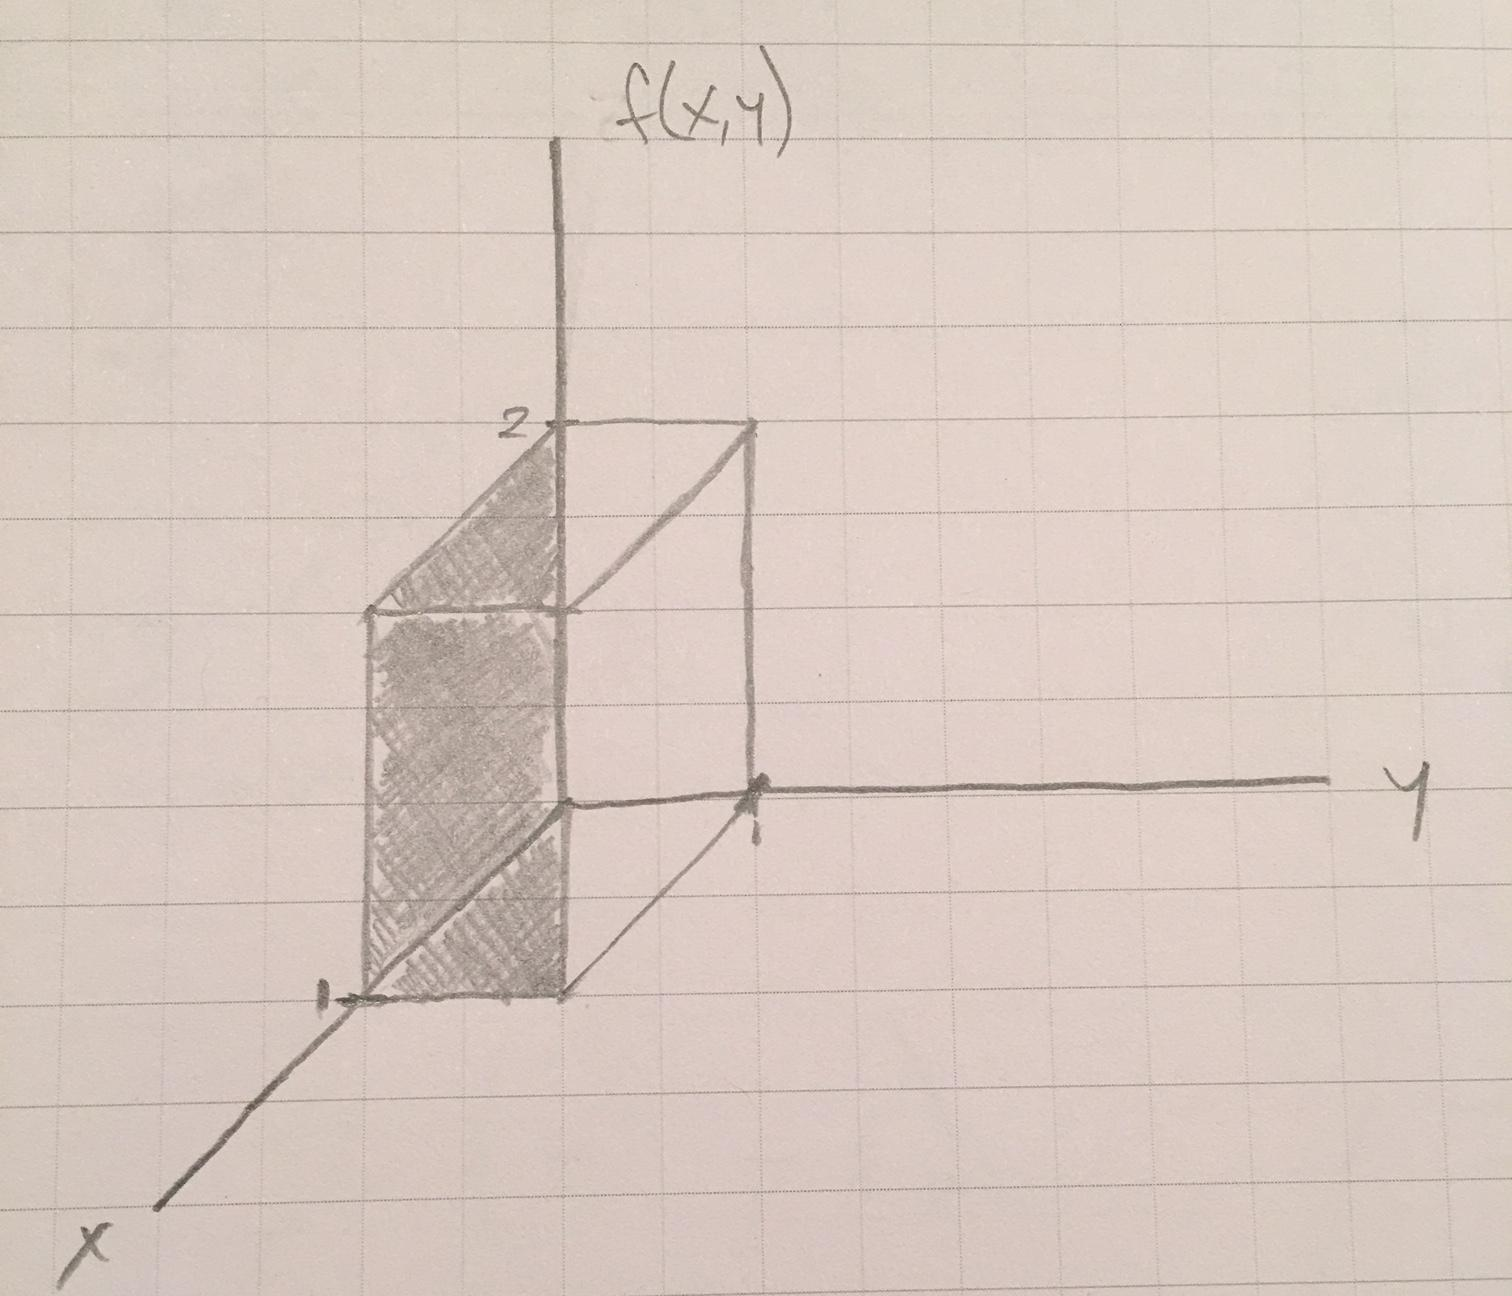
\includegraphics[scale=.2,keepaspectratio=true]{./images/graph1.jpg}
	% graph1.jpg: 1512x1296 pixel, 72dpi, 53.34x45.72 cm, bb=0 0 1512 1296
      \end{figure}
      
      \begin{enumerate}
       %a
       \item
	$f_X(x) = \lint_0^x {2\ dy} = 2y \Big|_0^x = 2x, 0 \le x \le 1$
	
	$f_Y(y) = \lint_y^1 {2\ dx} = 2x \Big|_y^1 = 2 - 2y = 2(1-y), 0 \le y \le 1$
       
       %b
       \item
	$\mu_X = \lint_0^1 {x f_X(x)\ dx} = \lint_0^1 {2x^2\ dx} = \dfrac{2x^3}{3} \Big|_0^1
	  = \dfrac{2}{3}$ 
	  
	$\mu_Y = \lint_0^1 {y f_Y(y)\ dy} = \lint_0^1 {2y - 2y^2\ dy} = 
	  \left[y^2 - \dfrac{2y^3}{3}\right]_0^1 = \dfrac{1}{3}$
	  
	$\sigma_X^2 = \lint_0^1 {x^2 f_X(x)} - \mu_X^2 = \lint_0^1 {2x^3\ dx} - \mfrac{2}{3}^2= 
	  \dfrac{x^4}{2} \Big|_0^1 - \dfrac{4}{9} = \dfrac{1}{18}$
	  
	$\sigma_Y^2 = \lint_0^1 {y^2 f_Y(y)} - \mu_Y^2 = \lint_0^1 {2y^2 - 2y^3\ dy} = 
	  \left[\dfrac{2y^3}{3} - \dfrac{y^4}{2}\right]_0^1 = \dfrac{1}{6}$
	  
	$Cov(X,Y) = E(XY) - \mu_X \mu_Y = \lint_0^x \lint_y^1 {2\ dx\ dy} - \dfrac{2}{9} = 
	  \lint_0^x [2x]_y^1 dy - \dfrac{2}{9} = \lint_0^x {2 - 2y\ dy} - \dfrac{2}{9} \\ = 
	  [2y - y^2]_0^x - \dfrac{2}{9} = 2x - x^2 - \dfrac{2}{9}$
	  
	$\rho = \dfrac{Cov(X,Y)}{\sigma_X \sigma_Y} = \dfrac{2x - x^2 - 2/9}{1/108}$
       
       %c
       \item
	$E(Y|x) = \lint_0^1 {y \dfrac{f(x,y)}{f_X(x)}\ dy} = \lint_0^1 {y\mfrac{2}{2x}\ dy}
	= \dfrac{y^2}{2x}\Big|_0^1 = \dfrac{1}{2x}$
      \end{enumerate}

     \addtocounter{enumi}{3}
     
     \newpage
     %17
     \item
      \begin{enumerate}
       %a
       \item
	Region for which $f(x,y) > 0$
	\begin{figure}[h!]
	  \centering
	  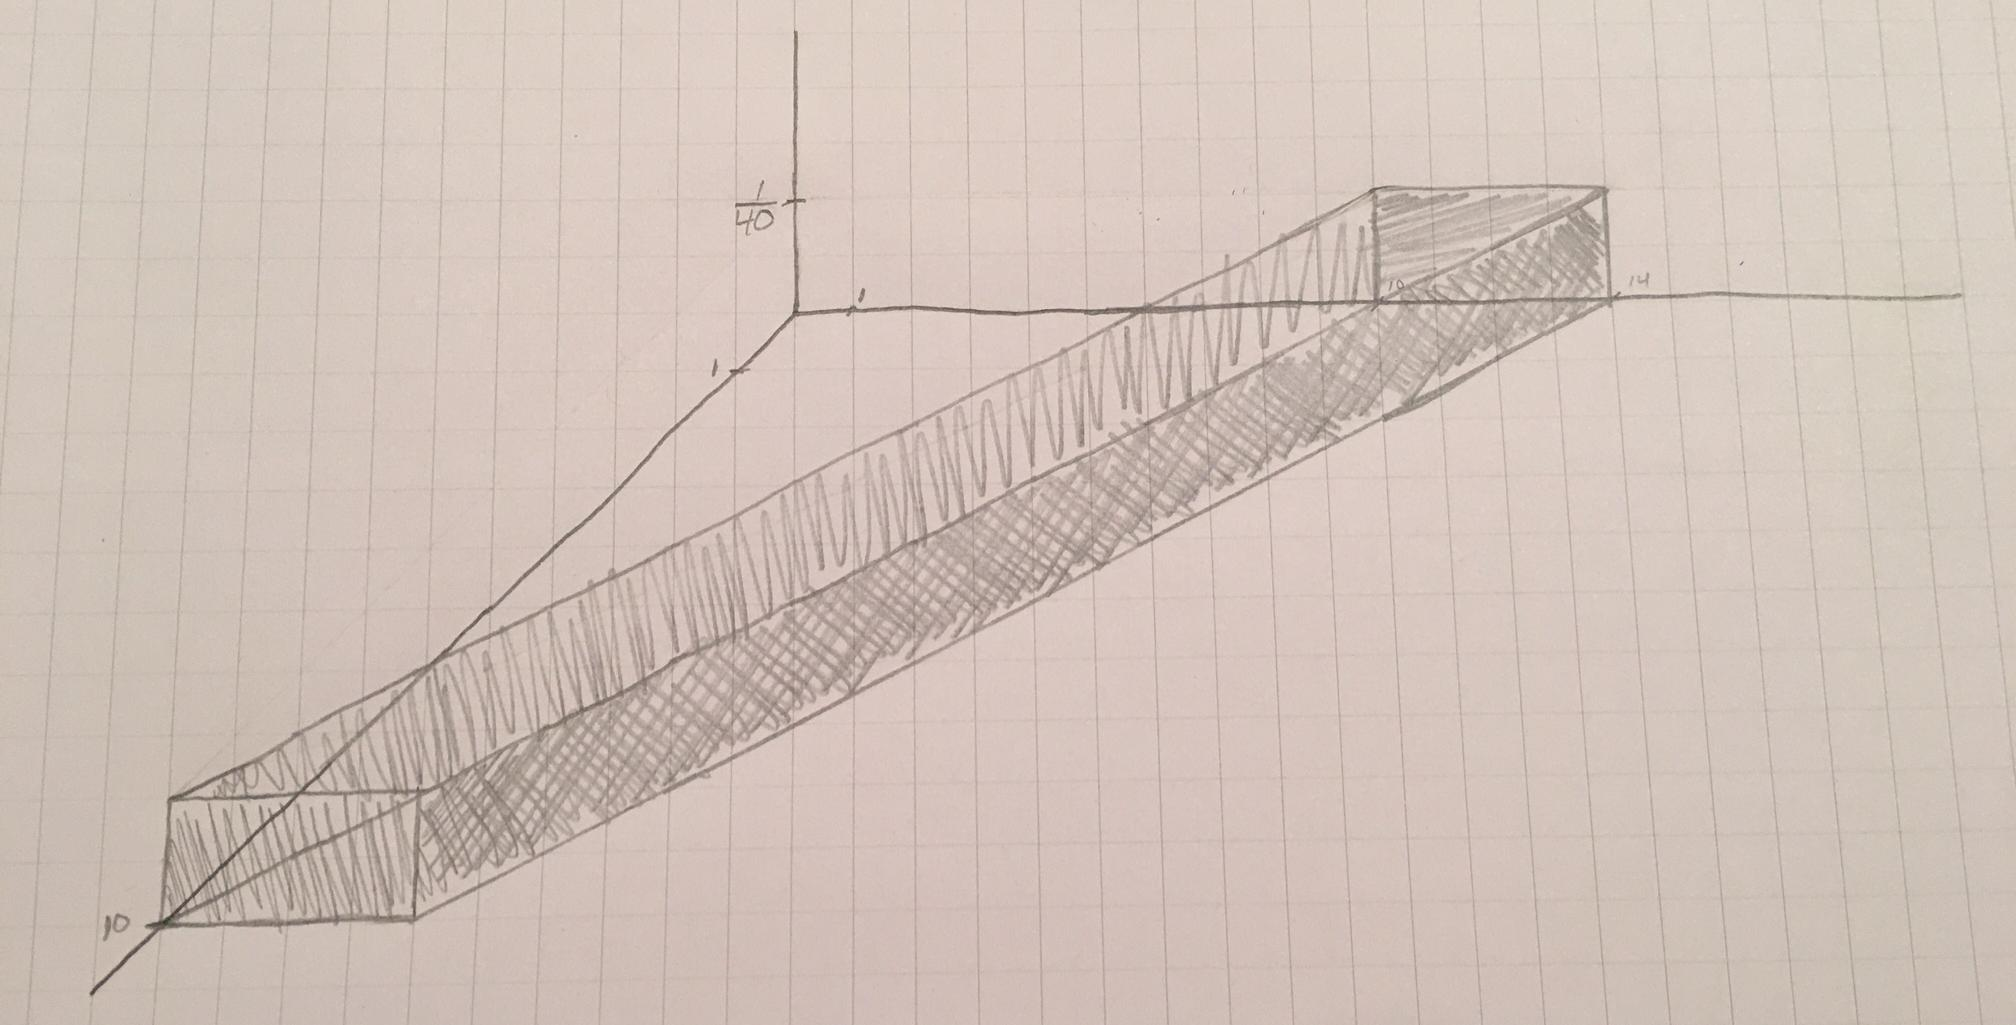
\includegraphics[scale=.2,keepaspectratio=true]{./images/graph2.jpg}
	  % graph2.jpg: 2016x1025 pixel, 72dpi, 71.12x36.16 cm, bb=0 0 2016 1025
	\end{figure}
       
       %b
       \item
	$f_X(x) = \lint_{10-x}^{14-x} {\dfrac{1}{40}\ dy} = 
	  \left[\dfrac{y}{40}\right]_{10-x}^{14-x} = \dfrac{14-x}{40} - \dfrac{10-x}{40} = 
	  \dfrac{4}{40} = \dfrac{1}{10}, 0 \le x \le 10$
       
       %c
       \item
	$h(y|x) = \dfrac{f(x,y)}{f_X(x)} = \dfrac{1/40}{1/10} = \dfrac{1}{4}
	  , 10-x \le y \le 14-x\ \text{for}\ 0 \le x \le 10$
       
       %d
       \item
	$E(Y|x) = \lint_{10-x}^{14-x} {y \dfrac{1}{4}\ dy} = 
	  \left[\dfrac{y^2}{8}\right]_{10-x}^{14-x} = \dfrac{(14-x)^2}{8} - \dfrac{(10-x)^2}{8} = 
	  \dfrac{196 - 28x + x^2 - 100 + 20x - x^2}{8} \\ 
	  = \dfrac{96 - 8x}{8} = 12 - x$       
      \end{enumerate}      
     \addtocounter{enumi}{1}
     
     %19
     \item
      \begin{enumerate}
       %a
       \item 
	We know that, $h(y|x) = \dfrac{f(x,y)}{f_X(x)}$. We are also given that $h(y|x) = 
	\dfrac{1}{x^2}$ and $f_X(x) = \dfrac{1}{2}$. Therefore,
	$$f(x,y) = \dfrac{1}{x^2}\mfrac{1}{2} = \dfrac{1}{2x^2}, 0 < x < 2, 0 < y < x^2$$
       
       %b
       \item
	$f_Y(y) = \lint_{y^{1/2}}^2 {\dfrac{1}{2x^2}\ dx} = -\dfrac{1}{2x} \Big|_{\sqrt{y}}^2 =
	  \dfrac{1}{2\sqrt{y}} - \dfrac{1}{4}, 0 < y < 4$
       
       %c
       \item
	$E(X|y) = \lint_{\sqrt{y}}^2 {x \mfrac{2\sqrt{y}}{x^2(2-\sqrt{y})}\ dx} = 
	  \mfrac{2\sqrt{y}}{(2-\sqrt{y})} [\log{x}]_{\sqrt{y}}^2 = 
	  \mfrac{2\sqrt{y}}{(2-\sqrt{y})} \log{\dfrac{2}{\sqrt{y}}}$
       
       %d
       \item
	$E(Y|x) = \lint_0^{x^2} {y \mfrac{1}{x^2}\ dy} = \dfrac{1}{x^2} \mfrac{y^2}{2}\Big|_0^{x^2}
	= \dfrac{x^2}{2}$
      \end{enumerate}
    \end{enumerate}
\end{document}